\documentclass[conference]{IEEEtran}
\IEEEoverridecommandlockouts
\usepackage{cite}
\usepackage{amsmath,amssymb,amsfonts}
\usepackage{algorithmic}
\usepackage{graphicx}
\usepackage{textcomp}
\usepackage{xcolor}
\def\BibTeX{{\rm B\kern-.05em{\sc i\kern-.025em b}\kern-.08em
		T\kern-.1667em\lower.7ex\hbox{E}\kern-.125emX}}
\begin{document}
	
	\makeatletter
	\newcommand{\linebreakand}{%
	\end{@IEEEauthorhalign}
	\hfill\mbox{}\par
	\mbox{}\hfill\begin{@IEEEauthorhalign}
	}
	\makeatother
	
	
	
	\title{Smart Shopping Cart System and Developing Shortest Path Using A star Algoritham\\
		%{\footnotesize \textsuperscript{*}Note: Sub-titles are not captured in Xplore and should not be used}
		%\thanks{Identify applicable funding agency here. If none, delete this.}
	}
	
	\author{\IEEEauthorblockN{Tarun S}
		\IEEEauthorblockA{\textit{Dept. of Computer Science (UG Student)} \\
			\textit{P.E.S. Institute of Technology and Management}\\
			Shivamogga, India \\
			tarun21799@gmail.com}
		\and
		\IEEEauthorblockN{Mehantha M}
		\IEEEauthorblockA{\textit{Dept. of Computer Science (UG Student)} \\
			\textit{P.E.S. Institute of Technology and Management}\\
			Shivamogga, India \\
			mehanthamegham29@gmail.com}
		\linebreakand
		\IEEEauthorblockN{Priyanka CS}
		\IEEEauthorblockA{\textit{Dept. of Computer Science (UG Student)} \\
			\textit{P.E.S. Institute of Technology and Management}\\
			Shivamogga, India \\
			priyankasshivraj1@gmail.com}
		\and % <------------- \and with a line-break
		\IEEEauthorblockN{Savina Gowda}
		\IEEEauthorblockA{\textit{Dept. of Computer Science (UG Student)} \\
			\textit{P.E.S. Institute of Technology and Management}\\
		Shivamogga, India \\
			savinagowdahnr@gmail.com}
		\linebreakand
		\IEEEauthorblockN{Mr. Puneeth B H}
		\IEEEauthorblockA{\textit{Dept. of Computer Science Engineering(Assistant Professor)}\\
			\textit{P.E.S. Institute of Technology and Management}\\
			Shivamogga, India \\
			puneeth.bh02@pestrust.edu.in}
	}
	
	\maketitle

\begin{abstract}
In today’s technologically advanced world, the majority of shoppers must wait in line to do their grocery shopping because it takes a long time. If a weekend or any promotional deals are announced, a large crowd will gather in the supermarket where barcode-based billing procedures require customers to wait in long lines. The products are also difficult to locate in the supermarket. In this regard, the Internet of Things (IoT)-based smart shopping cart is suggested which avoids the line at the checkout counter. The customer can quickly modify the shopping list via the mobile application. The server receives wireless shopping information after which billing is generated automatically. The goal of this experimental prototype is to get rid of laborious shopping procedures and service quality problems.\\
\end{abstract}

\begin{IEEEkeywords}
RFID(Radio-frequency identification), Smart application, Bluetooth module, Zigbee module, Arduino microcontroller, LCD display, A star Algoritham.
\end{IEEEkeywords}

\section{Introduction}
\begin{itemize}
	\item The Internet of Things (IoT) refers to an arrangement of interrelated, web associated objects that can gather and move information over a remote organization without human intercession.
	\item When something is associated with the web, that implies that it can send data or get data, or both. This capacity to send and additionally get data makes things "Smart".
	\item Our framework will want to foresee client interest in light of the past shopping client information and with the assistance of IoT, our framework will want to monitor every one of the items shopped and will want to give item data and vital subtleties on a client cell phone.
\end{itemize}	
     A shopping center is where individuals get their everyday necessities going from food items, clothing, electrical appliances, and so forth the time clients have issues in regards to the deficient data about the item marked down and misuse of pointless time at the charging counters\cite{b5}. Now and then clients deal with issues in regards to fragmented data about the item and holding up at the charging counters. Henceforth improvement is needed in the conventional charging framework to work on the nature of looking for clients. With this framework, the client will have data about the cost of each examined thing and the absolute cost of the thing. This will save the time needed in shopping centers. A cell phone with an android application is utilized here. The filtered items are consequently charged in the android application, accordingly essentially diminishing turnaround time\cite{b6}.\\
	Fast and simple payment of bills in the supermarket is one of the fantasies which each customer envisions of. so we will propose a "SMART SHOPPING CART" here we will utilize an RFID sensor. The main target of IoT is to screen individual items and the environment wirelessly. This introduces electronic tags connected with individual items. At the point when these tags become in the scope of the reader, it reads the stored data of the object wirelessly which is known as RFID innovation\cite{b1}. RFID assumes a vital part in the utilization of IoT. It comprises of three parts, for example, RFID tags connected to the object that contains personality or information about an item, RFID Reader reads the tags. The significant utilization of RFID innovation is to follow the item\cite{b1}-\cite{b8}.
	

\section{Electronic Components :}

\subsection{RFID Reader :}
The RFID reader is utilized to accumulate data from the RFID tag which is utilized to follow individual items radio waves are utilized to move information from tag to reader\cite{b1}.
   

\subsection{RFID tag :}
Radio-frequency identification (RFID) uses electromagnetic waves to identify the tags attached to the products. RFID provides storage to data. it is utilized to recognize, track, and communication with things and individuals. RFID labels are smart labels that can store a scope of data information from serial numbers\cite{b1}.


\subsection{Arduino uno microcontroller :}

Arduino Uno is a Microcontroller board named Arduino Uno given the ATmega328 series regulator. You can handle your board on how to treat sending a bunch of guidelines to the microcontroller on the board\cite{b7}. It works with the designers and software engineers with a coordinated advancement environment in which various tasks can be performed without any problem. Like composition, incorporating, and transferring code to the microcontroller\cite{b8}.

\subsection{Bluetooth module :}
Bluetooth module HC-06 is intended for building up short-range remote information correspondence between two microcontrollers or frameworks\cite{b1}-\cite{b2}. The module chips away at Bluetooth 2.0 correspondence convention and it can go about as a slave gadget. This is the least expensive technique for remote information transmission and more adaptable contrasted with different strategies and it even can send records at an accelerate to 2.1Mb/s.

\subsection{LCD display}
The most ordinarily utilized LCDs found in the market today are 1 Line, 2 Line, or 4 Line LCDs which have just 1 regulator and backing all things considered of 80 characters, while LCDs supporting over 80 characters utilize 2 HD44780 regulators. Most LCDs with 1 regulator has 14 Pins and LCDs with 2 regulator has 16 Pins (two pins are extra in both for backdrop illumination LED associations)\cite{b2}.

\subsection{QR scanner :}
QR codes are fit for putting away loads of information. Be that as it may, regardless of the amount they contain, when checked, the QR code allows to permit the client to get to data instantly\cite{b2}.QR codes are often used to follow data about items in a production network and because a huge number have implicit QR readers they are frequently utilized in showcasing and promoting efforts.

\section{Problem Statement}
	Design and implement IoT and machine learning techniques to predict the customer interest in shopping and provide the detailed bill of the products present in the trolley using RFID technology. 
	


\section{Literature Survey :}
In this paper\cite{b1}, RFID offers types of assistance to the buyer for example show the item data, past shopping history, dealing with a current shopping list, item advancements, exceptional offers, item area to the shopper, and RFID-based login process for better security. At the point when items draw close to the RFID reader in the shopping basket. The purchaser can cooperate with item data. This data is separated by portable applications from backend data sets put away in the waiter framework. The buyer can likewise look for the ideal item area in the general store through collaboration with a static guide of the store. The buyer can likewise collaborate with past shopping history, item advancements, and exceptional offers. That assists the shopper with recalling items to buy, dealing with the shopping list, and can get the best items as per their inclinations\\

In this paper\cite{b2}, Shopping, in reality, includes both genuine articles and brilliant items. Items arrangements and openness are significant for store shopping what item stores show in plain view. they involved sensors for their streetcar and furthermore remote correspondence to impart and a Barcode Scanner for checking the standardized identification on the item and will show the cost of the item.
A grocery store is where individuals come to buy their day by day involving items and pay for them. So there is a need to work out the all-out items and aggregate sum. Here we use RFID labels to diminish the time and decrease work costs by moving to self-administration. Likewise use Zigbee innovation which is a low information rate, minimal expense, low power utilization innovation.\\

In this paper\cite{b3}, shopping baskets can be utilized in shopping stores, wherein every item in the store will be furnished with RFID for the ID of items. This smart shopping basket will likewise have an LCD screen joined to it which will inform clients about item costs, limits, offers, and the absolute bill. Predictable Wi-Fi association with the shop's waiter is very fundamental. The way that a cart is supportive of effectively creating charging data liberates the staff from redundant checking and consequently expands the functional productivity of the framework.\\

In this paper\cite{b4} author gave an explanation about how to predict the customer needed product using machine learning algorithms. Using these algorithms we can predict the customer needed items before he/she is going to buy. Based on previous customer history like product names, dates, costs, and applying some machine learning algorithm we can predict the customer needed item in the shopping mall.\\

In this paper\cite{b5} they explained that a trolley is equipped with an
RFID reader and LCD screen. when a product is placed in a trolley it detects
the code automatically, the item name and cost will be displayed on the LCD
and also the cost gets added to the total bill. The billing of a product or the
information of the product will be passed to the central billing unit via the
Zigbee module. Analysis between barcode and RFID has been done in this
paper where the RFID has to strengthened effectiveness in many fields. The
unit cost for standardized tags is affordable and it can be printed specifically to
the items or boxes. Python language is used by Rasberry Pi for connecting with
the RFID reader. The tags used in this project have only one side detection
so they are attached circularly to avoid non-detection. when the evaluation is
done with a single shopping cart with distinct items\\

In this paper\cite{b6} they have given that the RFID attached to the
shopping cart helps to detect the presence of users in the shopping market.
Here smartphone is used as a barcode scanner. When the smartphone scan the
product the description of the product is sent to the audio and this description
will be displayed on the LCD which is attached to the smart trolley. Once the
customer finished his shopping then he needs to press the button on the trolley
the total bill will be sent to the computer using NRF24L01.\\

In this paper\cite{b7}, this system will provide on spot scanning of the items and also shows the price details of the items on LCD connected to the trolley. This allows the customer to compare the total price with their 
budget in the pocket before billing. After customers shopping is done and they move near the billing counter, the data from the LCD is going to transfer to the billing counter computer through NRF24|01. In
this way, it may save the time of the customer as well.\\

In this paper\cite{b8}, they have designed and developed a smart cart system. This project helps customers to not wait in the queue and wait for their turn for scanning of products. Where the trolley is connected 
to the mobile application of the customer. The RFID reader in the trolley scans the products that are added to the cart. The list of products, amount and total billing will be displayed. The payment can be done 
through various payment options provided or through the cash counter. The trolley can be moved throughout the mall through the application, it need not be pushed manually with the help of the Bluetooth module\\

Many people have consistently visualized and built up an upheaval to help society's needs as far back as the start of humanity. The basic reason for headway in innovation has been in limiting tasks and making regular tasks simpler and quicker, regardless of the different spaces accessible. A remarkable task on which people are discovered spending significant measure of time is shopping. Initially, barcode systems were used but after some years it also started to have issues like an increasing queue, etc. so to overcome these issues a concept of the smart cart using RFID technology was proposed.\\

The performance of the Internet of Things(IoT) based automated trolley system was reported in \cite{b9}. To ease line in shopping mall framework is utilized by utilizing RFID module. The RFID reader will read the RFID tags set on the product when the product is added to the trolley. In this event, the customer needs to remove any product then they should remove that product from the trolley. In LCD which is connected to the trolley will show the information of the expelled product like name, cost, and the absolute bill with the help of the Xampp server the bill will be sent to the cashier.\\


In paper\cite{b10} authors work on a method for an automatic billing system in shopping malls. The basic thought behind this project is to decrease the problem in a shopping mall so that no need to wait in a long queue for hours and no one has to waste their time in billing. In this proposed system the authors make use of RFID technology for billing the products which are then integrated with the ARDUINO microcontroller. In this project, they haven't properly mentioned the type of ARDUINO. And also the bill will be then sent to the cashier with help of a USB and the bill can be printed on the spot. DipTrace is used for making the circuit, It is open-source software that enables us quick and easy design of circuits. They used Visual Basic Software to make admin's portal and with the help of Java programming language, they have created GUI for their system. When you add something to the trolley the RFID reader will scan and the bill gets generated. After shopping the customer has to press the bill button and then the trolley gets connected to the computer and transfers the bill.\\ 

In this paper\cite{b11}they have used EM-18 RFID scanner module. Using this RFID reader 125kHz tags can be read. It offers a serial output and contains a range of approximately 8-12 cm. It has an inbuilt antenna and is connected to the computer system with the assistance of RS232. This RFID module is capable of handling multiple tags at a time also range is very less so it will not get in contact with another trolley. The RFID readers use the big tags with a range of 125KHZ which can be exposed by the EM-18 Module. This shows the real-time billing and can even delete the item which is not required by pressing the delete button. In this, the author has used ARDUINO Uno which is the cheapest and most efficient model in the market. It contains everything required to support the micro-controller merely connect it to an applicable wall power adapter using a USB cable. If the products are scanned it will start generating the bill and products can be removed if needed. However, they have not mentioned how the receipt will be transferred to the billing section as they also want to keep the database updated for refilling the stocks.\\

In this paper\cite{b12} they have proposed a system where every product would be read by scanning tag as it is added to trolley. Even the expiry date of the product gets displayed along with the information of the product. The most intense and clear system has a unique id connected to each product as soon as the product is read by the reader it automatically generates the information regarding the items on the screen. Micro-controller memory is used to store the product id and its details. As soon as the data information about the items is displayed on the LCD screen the bill has been transferred to the system computer via GSM/GPRS module.  A per the testing, when the item is added or removed from the trolley, the cart can precisely and perfectly read the information. The metal outside the cart restricts the signal to a high degree that when the reader is inside the trolley, no other products other than the cart are being read. This perfectly shows that the product into a smart trolley will not be damaged or read by a nearby cart accidentally.\\

In paper\cite{b13} the authors came up with the system which consists of GSM, RFID, Automatic Billing, OTP, ZigBee, PIC, etc. In this project, the products can be read by the RFID reader, and the total information of the product is displayed on the LCD screen. They have specified this paper because they have added some additional features to an existing system. Like right now, the thing can be read by the RFID peruse, and the aggregate of the thing is displayed on the LCD screen. this paper has been portrayed since they included some extra highlights in the existing framework.
Like in the present system product weight and name appeared in plain view; in the task, that thing weight is not exactly put away weight, at that point signal will blare. If there is any unauthorized task being conducted then the customer would either get a buzzing sound or a text message via the GSM module. The LED system is used to make customers alert about unauthorized activity.\\

Paper\cite{b14} describes the designed smart shopping trolley that used the RFID technology to fetch the information of products already present in the database and also provides an automated billing system using RFID and Zigbee communication. A localization algorithm(Fast map algorithm) is used to find the particular product location. Each product will have an RFID tag and I contain a unique identification number, product details like nutritive contains expiry date, etc. Each cart has a PID(Product Identification Device) specifically containing a micro-controller, LCD, an RFID reader, Keypad, Buzzer, IR add sensor, IR remote sensor, RF transceiver module. The power supply of 12V is used as the input voltage for different components used in the system.16*4 LCD will display the information when the RFID reader reads the products in the cart.IR add sensor is used to add the price when we add the product into the cart and IR remove sensor used to deduct the price of the product when we remove it from the cart.\\


Paper\cite{b15} designs a shopping cart made up of technical components like -OLED, Buttons, Bluetooth Transceiver/ESP8266, NFC reader, and microcontroller. Here they use NFC protocol for wireless communication it transfers the shopping list from the product to the basket. It provides peer-to-peer communication data transfer.ESP8266 wifi module used to establish communication between hardware components like send and receive data. Using the wifi module we can store the data in a database like a firebase.OLED is used to link the customer with this technology. It provides the user with details about the item in the cart and the total bill. In this project, the microcontroller they used is Arduino UNO R3 used to analyze the information in the tag and update accordingly.\\


Paper\cite{b16} Authors have designed a construct of a shopping trolley, here they mainly used mobile applications on the mobile phone and a weighted sensor system composed of a load cell module linked to a load cell amplifier HX711 module. The total weight of the items in the shopping basket is recorded in the cloud servers. after being transmitted to the ESP8266 NodeMCU via Wi-Fi Network. The product information will be shown after the product is scanned by the RFID reader.\\


Paper\cite{b17} describes the implementation of a smart shopping cart using an RFID code system, automatic lock system, EEPROM, Zigbee Module, IR coupling, HC-12, Cartesian system. The RFID reader attached to the cart reads the product when it drops into the trolley and displays the information in LCD Display.EEPROM stores the information and sends it to the billing counter. There will be securely attached to the product if anyone takes the product outside the shopping mall without scanning the security alarm will be alerted at the door.LCD also shows the total bill of the product.\\





In this paper\cite{b18}, they gave that the customer no need to stand in front of the billing counter to pay the bill that he has purchased. And the trolley will act as a smart trolley it will send the information of the product and total bill sent to the central system by scanning the product using an RFID reader. It consumes the customer’s time and increases customer satisfaction.\\

In this paper\cite{b19}, they have given that shopping trolley contains hardware components like Arduino Mega 2560 microcontroller, RFID Reader, ultrasonic sensor, Auto-calibrating sensor, and motor driver,12V acid battery.RFID. The reader reads the tag which is on the product, then the information of the product will be stored in the Arduino Mega 2560 microcontroller then the information sent to the smartphone using a Bluetooth module. Ultrasonic sensors are used to detect an obstacle and their avoidance. The motor driver helps to drive the shopping trolley and the movement is controlled by the smartphone.\\

In this paper\cite{b20}, they have given that the RFID attached to the shopping cart helps to detect the presence of users in the shopping market. Here smartphone is used as a barcode scanner. When the smartphone scan the product the description of the product is sent to the audio and this description will be displayed on the LCD which is attached to the smart trolley. Once the customer finished his shopping then he needs to press the button on the trolley the total bill will be sent to the computer using NRF24L01.\\

In this paper\cite{b21}, they proposed architecture for passive RFID product tracking. The author only believes that only by involving users, companies will be involved in IoT ecosystems. They also proposed a business model a global tracking system for proposed products in which users could obtain benefits from recycling activities. Even in the proposed platform, the manufacturer includes its identity within the product code in the RFID label attached to the product. The service running in the RFID reader only has to interpret the printed RFID identity and invoke the method in the corresponding manufacturer service. And also explained the benefits and costs depending on the roles.\\

In this paper\cite{b22}, they explained that a trolley is equipped with an RFID reader and LCD screen. when a product is placed in a trolley it detects the code automatically, the item name and cost will be displayed on the LCD. The billing of a product or the information of the product will be passed to the central billing unit via the Zigbee module. Analysis between barcode and RFID has been done in this paper where the RFID has to strengthened effectiveness in many fields. The unit cost for standardized tags is affordable and it can be printed specifically to the items or boxes. To connect with the RFID Reader here they used python language in Rasberry Pi. The tags used in this project have only one side detection so they are attached circularly to avoid non-detection. when the evaluation is done with a single shopping cart with a distinct item.\\

In this paper\cite{b23}, they have created an automated central bill system for supermarkets and malls. After purchasing the bill is paid through credit/debit cards. To read the 8-bit data from the RFID reader here they used 8-microcontroller. They have used AT89S52 but the programmer needs to write a separate Embedded C program to send and receive data with EEPROM because AT89S52 does not have an inbuilt 12C protocol. This may create difficulty to write a program for programmers to synchronize with EEPROM. This can be overcome by using the microcontroller and microprocessors which have inbuilt 12C protocol features.\\

In this paper\cite{b24}, they have reported about a surveillance system in a shopping lab and analyzed the shopping behavior. Based on human tracking, tracking for different shoppers, and face localization they have designed and implemented a running prototype and tested the modules - motion detection, trajectory analysis. \\




\section{Architecture :}
\begin{figure}[htbp]
	\centerline{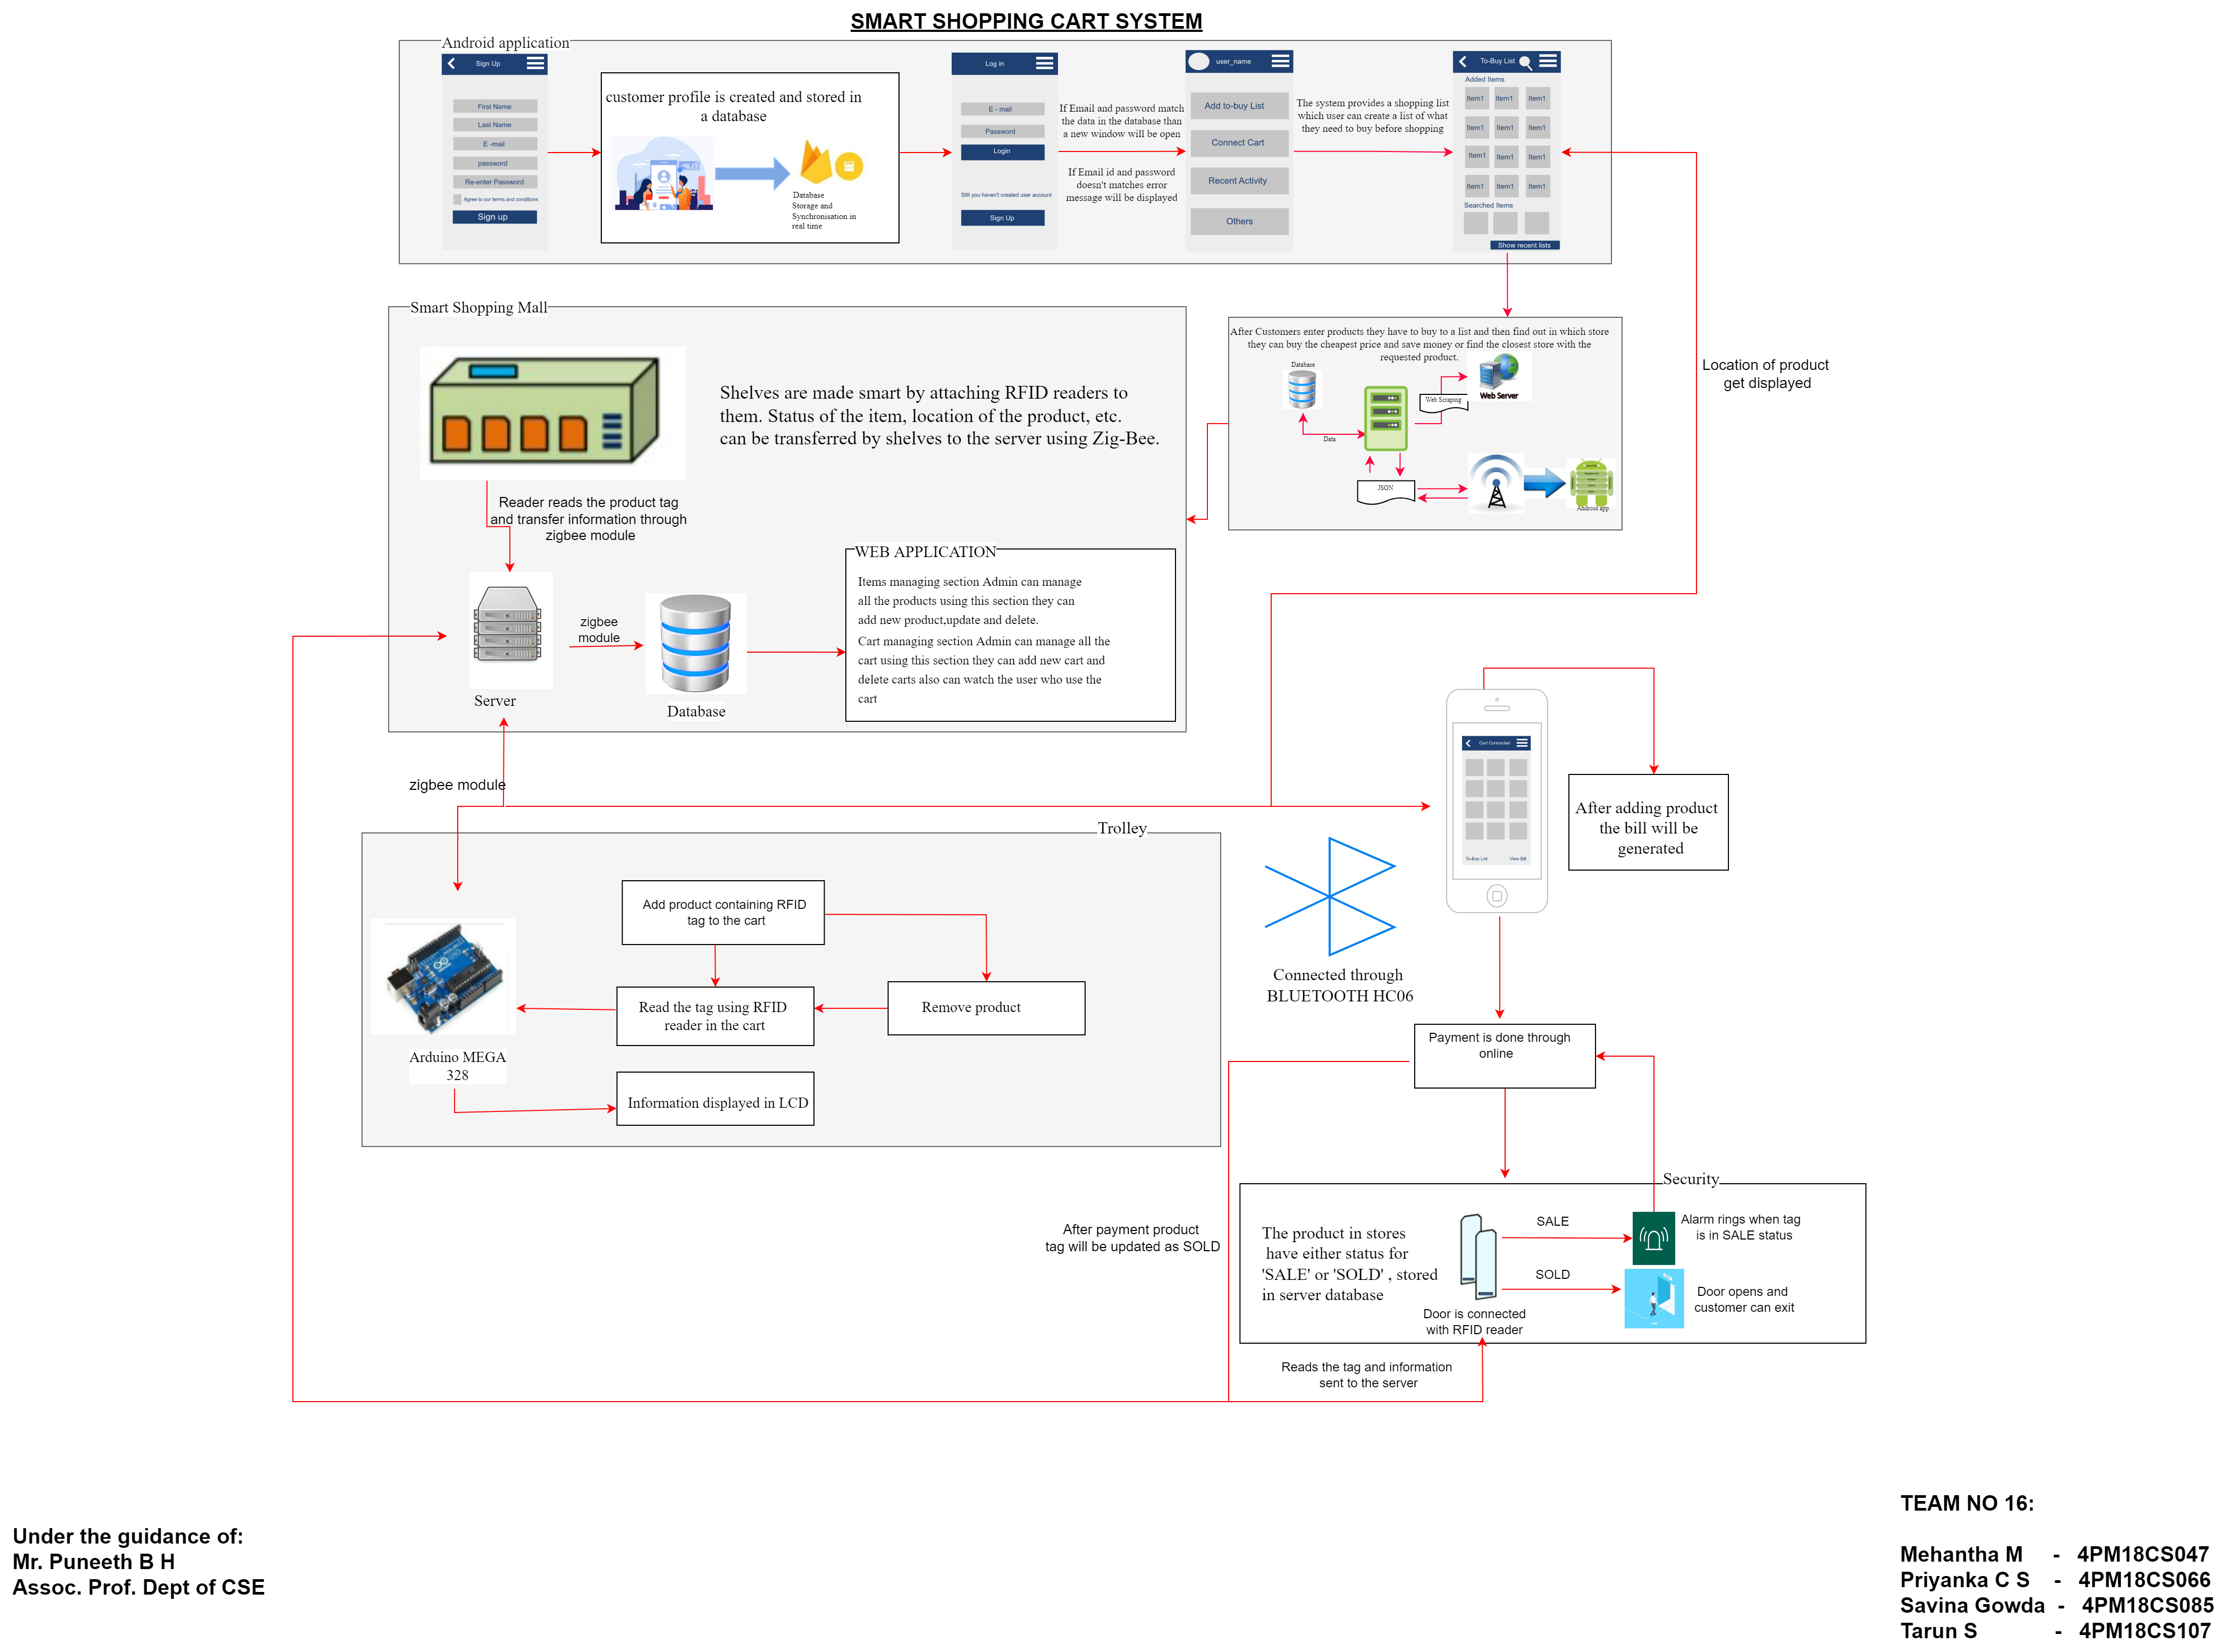
\includegraphics[width=100mm]{download}}
	\caption{Architecture}
	\label{fig}
\end{figure}
Initially, the customer login to the application and choose the shopping mall he wishes to visit to purchase the items. once the shopping mall is selected the application will provide the list of items available in the shopping mall. the customer will select the items he wishes to buy from the list and then the application will provide the shortest route to reach the shopping mall\cite{b4}. Based on customer mobile location the centralized server will get to know about the customer reached the shopping mall or not. once the customer reaches the shopping mall, inside the mall shelves are made smart by attaching an RFID reader to the shelves that will help to find a product location.. once the customer reaches the first product location then the application will sort the product list again based on the current location of the customer inside a shopping mall. Once the customer reaches the product location he will add the product to the trolley containing the RFID reader each product will have an RFID tag, the RFID reader will read the product tag and send a request to the centralized server to fetch details of the product and details will be displayed on an LCD screen attached to the trolley parallelly using Bluetooth module the product details will be updated in the mobile application along with a price\cite{b1}. Once all the products are added, the mobile application will display the list of items in the trolley along with price details and total cost of all the items to pay the bill that can be done by using unified payment interface ex: google pay, phone pay, etc... If in case if the customer wants to remove any items from the trolley he/she needs to make an RFID reader read the tag of that particular item, that will send a request to the server to delete the item and it will provide a delete option in the mobile application to remove and the list is updated along with the cost. the product in stores has either status as SALE or SOLD stored in a database server\cite{b3}. if any product is in sale status then a QR code will not generate an alarm will ring if all the products are in sold status then a QR code will generate and the customer can leave the mall\cite{b3}.

\section{Methodology :}
\begin{figure}[htbp]
	\centerline{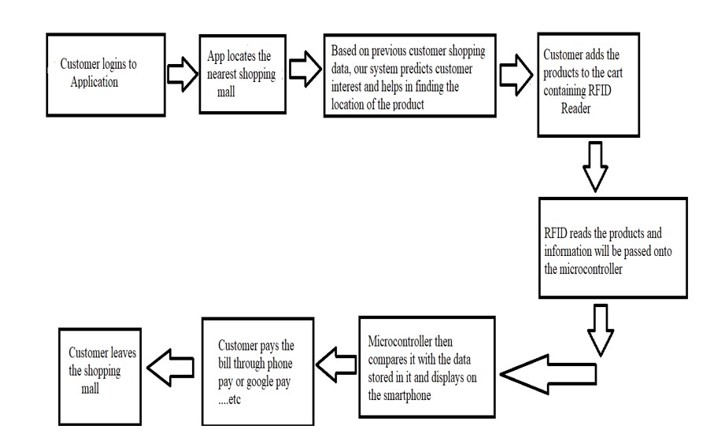
\includegraphics[width=80mm]{Flow_Digram}}
	\caption{Flow diagram}
	\label{fig}
\end{figure}
\begin{itemize}  
\item This application has Administrator,Moderators,Users.
\item The administrator is the super user of this application. Only admin have access into this admin page. Admin may be the owner of the shop. The administrator has all the information about all the users and about all products
\item A moderator is considered as a staff who can manage orders for the time being. As a future update moderator may give facility to add and manage his own products
\item A new user will have to register in the system by providing essential details in order to view the products in the system. The admin must accept a new user by unblocking him
\item Customer logins to the application
\item The app locates the nearest shopping malls
\item Based on previous customer shopping data, our system predicts customer interest and helps in finding the loca- tion of the product
\item Customer adds the products to the cart containing RFID Reader
\item RFID reads the products and information will be passed on to the microcontroller
\item Microcontrollers compare it  with the data stored in it and display it on the smartphone [7].
\item Customer pays the bill through phone pay or googles pay etc. . . .
\item The customer leaves the shopping mall.

\end{itemize}		

\section{Results}
\subsection{Objective 01}
When the device is switched on, the NodeMCU successfully connects to the Wi-Fi and the IP for the site is displayed on the LCD screen for about 30 seconds. After entering the IP in the web browser, a web page containing the products along with their quantities and prices is displayed in tabular form. All the product cards were successfully scanned and the confirmation was displayed on the LCD screen. On scanning the RFID card of a product, information about the product along with the cost is displayed on the LCD screen as well the web page is updated with its content. Also, the deletion of items was successful. After scanning the checkout card, the total bill is displayed on the LCD screen. The system successfully resets after pressing the ‘Reset’ push button.

\begin{figure}[htbp]
	\centerline{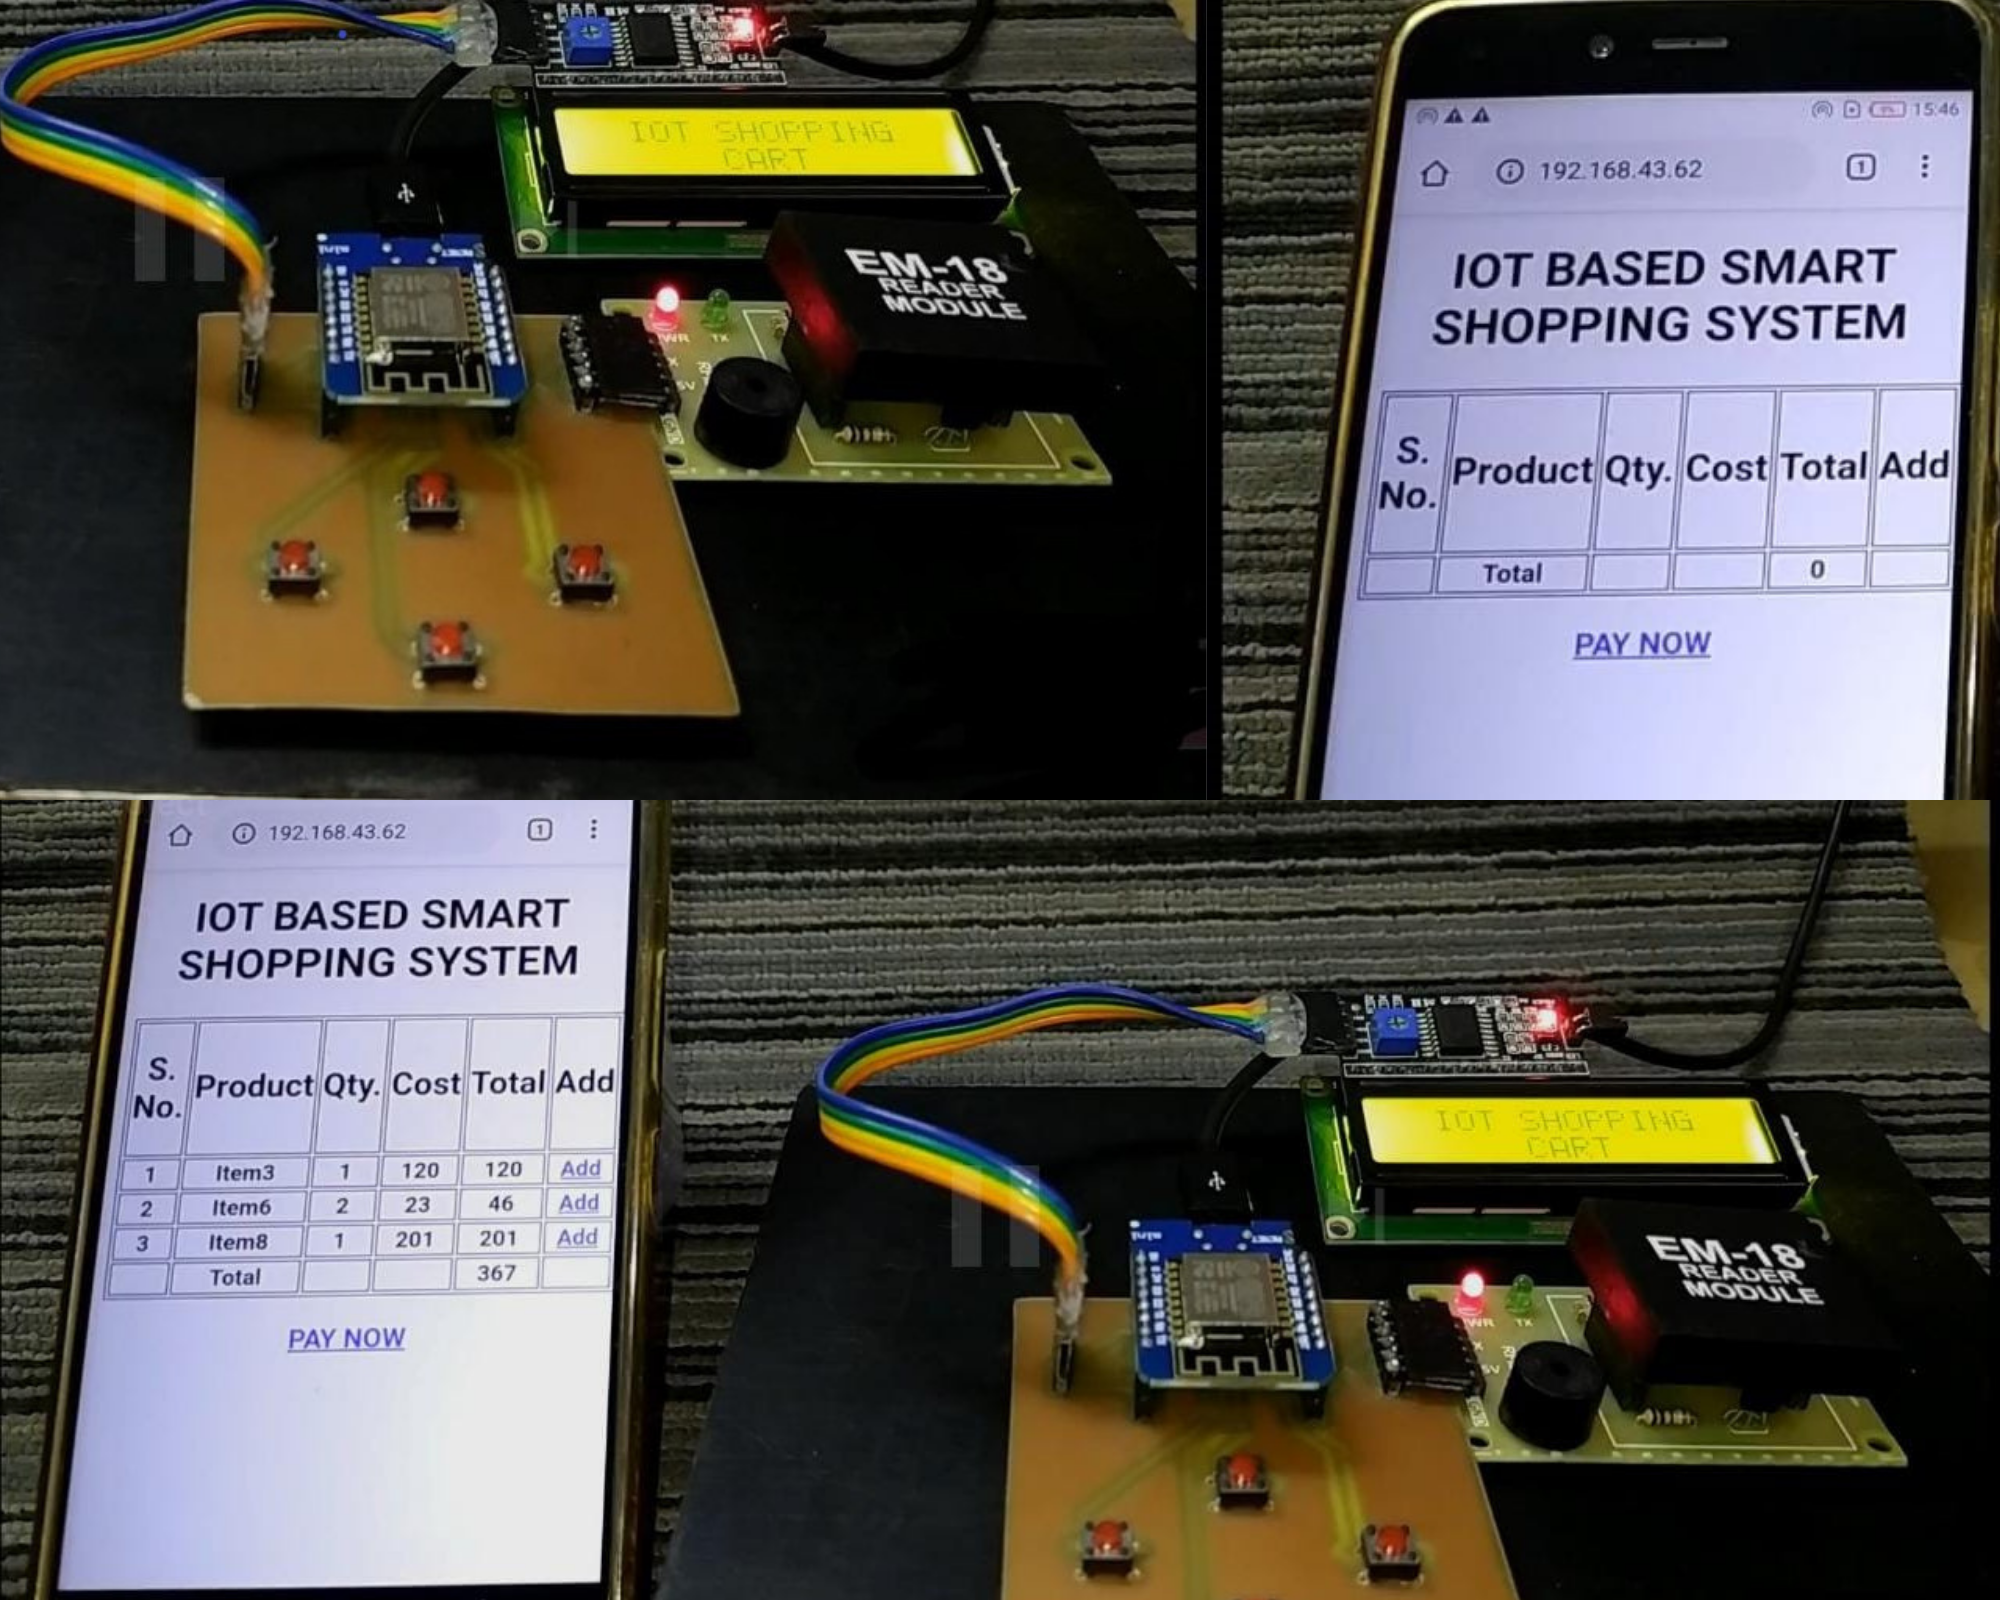
\includegraphics[width=80mm]{Iot}}
	\caption{Objectivi 01 Output}
	\label{fig}
\end{figure}



\begin{figure}[!htb]
	\centerline{\includegraphics[width=80mm]{iot-04}}
	\caption{Admin Page}
	\label{fig}
\end{figure}

\begin{figure}[!htb]
	\centerline{\includegraphics[width=80mm]{iot-05}}
	\caption{Inventory}
	\label{fig}
\end{figure}
\begin{figure}[!htb]
	\centerline{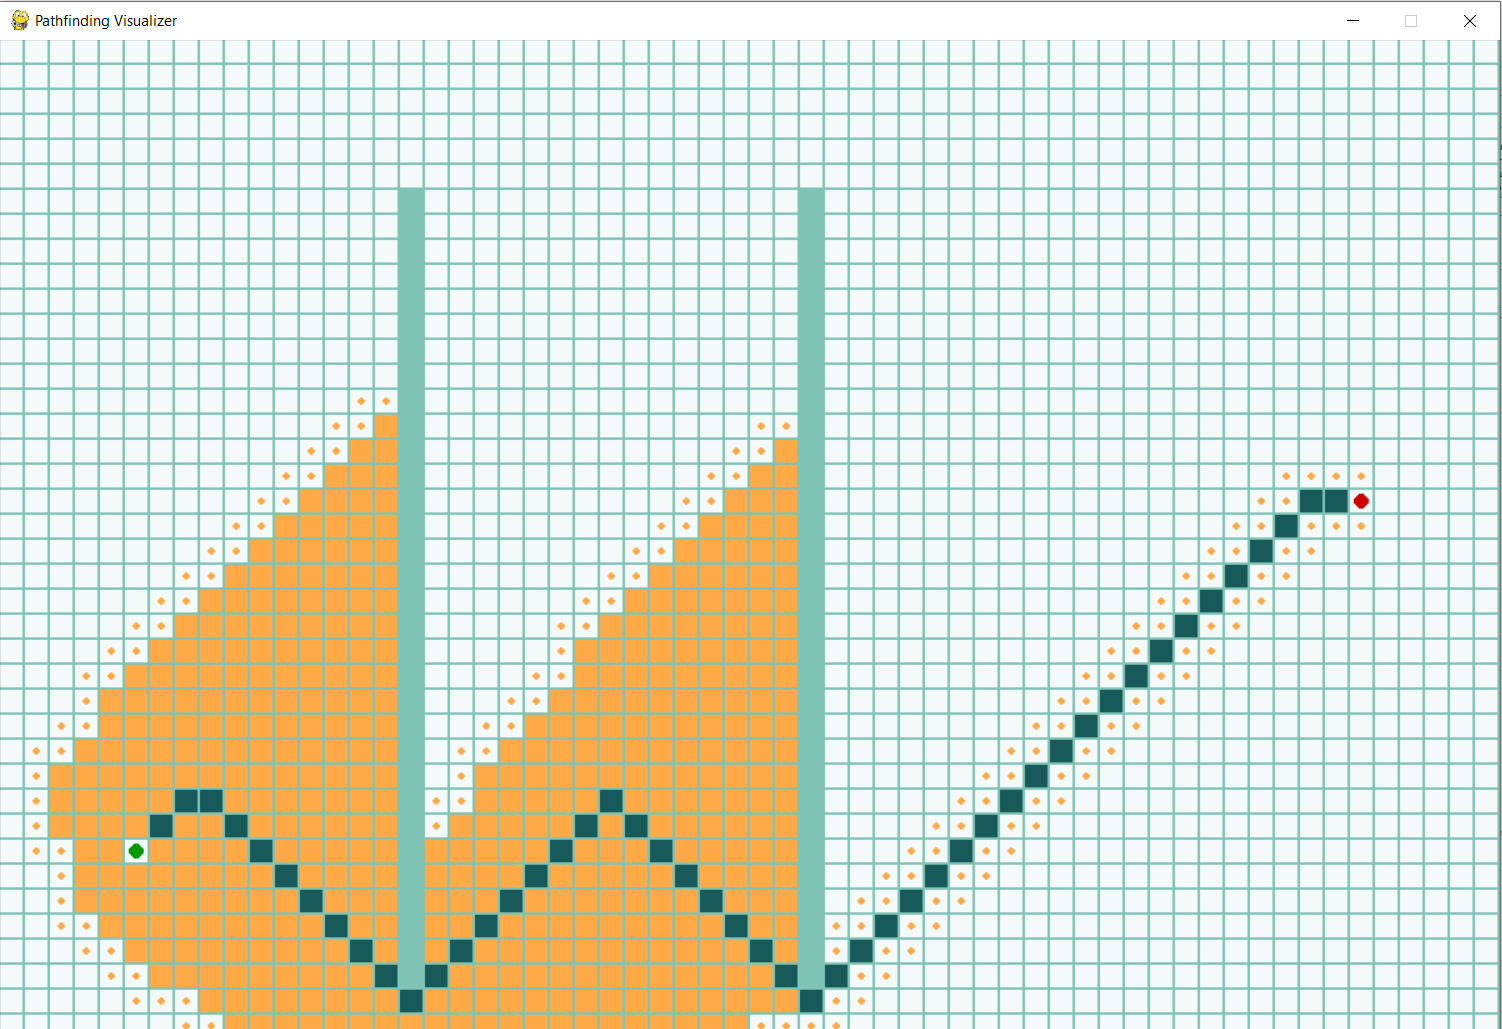
\includegraphics[width=80mm]{iot-06}}
	\caption{Developed Shortest Path Using A star Algoritham}
	\label{fig}
\end{figure}
\begin{figure}[!htb]
	\centerline{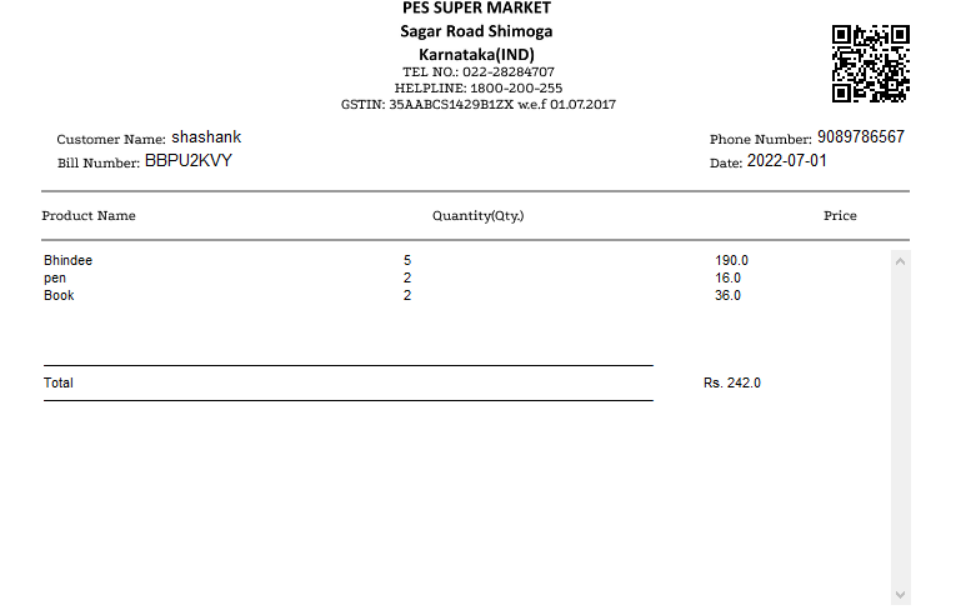
\includegraphics[width=80mm]{Image-07}}
	\caption{Total Bill with Unique QR Code}
	\label{fig}
\end{figure}

\subsection{Objective 02}
Creating an inventory database using python flask. Our platform offers shoppers
personalized shopping mall experiences, allowing them to create a product list and
discover products they want to buy every time they go shopping. The admin page allows the admin to add, or remove the product information and based on the customer
product list it will track the product and develop a shortest path based on the location of the product present in the shopping mall using A Star Algoritham.\\

\section{Conclusion :}
A smart shopping basket is made by involving IoT and machine learning this application is involved by clients in the shopping center to save a great deal of time in purchasing any products. This application assists with decreasing the labor in the shopping centers. In this undertaking[43-49], RFID is utilized as protected admittance for the thing which improves the observation execution. This execution starts with automated central billing in the shopping centers and grocery stores. with this, the clients never again need to stand by at a charging counter furthermore this is a less difficult cycle[5], for payment of bills their bought thing data gets moved to the central billing unit, and that installment of the bought things will be finished utilizing a unified payment interface.\\


\section*{Acknowledgment}

Smart Shopping Cart System Research was carried out as our 4th-year research in P.E.S. Institute of Technology and Management under VTU, Shivamogga, Karnataka. We are extremely grateful to our supervisors Dr. Likewin Thomas and Mr. Puneeth B H who shared their great knowledge, constant encouragement, and support making the pathway for the success of this research.\\


\begin{thebibliography}{00}
\bibitem{b1} IoT-based Smart Shopping Cart Using Radio Frequency Identification.IEEE Access 2016. 
MOBEEN SHAHROZ1, MUHAMMAD FAHEEM MUSHTAQ2, MAQSOOD AHMAD 1, SALEEM ULLAH1, ARIF MEHMOOD3, AND GYU SANG CHOI 4.

\bibitem{b2} Automated Shopping Trolley for Billing System. IJIRST june 2017 volume 4. 
Mrs. D. M. Yewale, Akshata Ujalambkar, Utkarsha kate, Priyanka shendkar.

\bibitem{b3} IoT Application on Smart and Secure Shopping System using RFID, Zig-Bee and Gossamer Protocol.IJET volume 4 issue3 may-june 2018. 
1Purva S. Puranik1 , Parikshit N. Mahalle2.

\bibitem{b4} Customer buying Prediction Using Machine-Learning 
Techniques: A Survey IRJET volume5 issue10 Oct 2018.
Mr. Shrey Harsh Baderiya1, Prof. Pramila M. Chawan2 .

\bibitem{b5} A Survey on Smart Trolley System Based on Android Application IJSRSET volume4 issue4 march 2018.  
Prarthana Bhandekar, Chanchal Tomar, Divyani Kasewar, Prof. Ansar Sheikh.

\bibitem{b6} A Survey Paper on Smart Trolley Using RFID Technology.IJFGCN volume13 2020 
1Ashutosh Walimbe, 2Vikrant Pagnis, 3Akshit Alva, 4ASidhesh Balapure, 
5Madhuri Karnik.

\bibitem{b7} Smart Trolley using Smart Phone and Arduino.JEES 2017
Harpreet Singh Bedi*, Nikhil Goyal, Sunil Kumar, and Avinash Gupta

\bibitem{b8}A Smart Trolley System using RFID.IJRESM volume2 issue4 april 2019 
Amruta Pokale1 , Kajal Pilane2 , Prakash D. Kshirsagar3.

\bibitem{b9}Priyanka S. Sahara, Anup Gade, Jayant Rohankar A Review on automated Billing for Smart Shopping System Using IOT International Informational engineering technology association 
\bibitem{b10}Sarika S. Pandey, Soumya R. Gupta, Meenaz M. Shaikh, Komal M. Rawat, Prof. Pravin Jangid, Prof. Ragini Mishra Smart Cart Using Arduino and RFID Volume: 05 Issue: 03 | Mar-2018
\bibitem{b11}Vaishali Rane, Krutik Shah, Kaushal Vyas, Sahil Shah, Nishant Upadhyay Smart Trolley Using RFID Volume: 06 Issue: 01 | Jan 2019
\bibitem{b12}Pritha N, Sahana S, Selvin Stephy N, Shiny Rose S, Annamalai S Smart Trolley System for Automated Billing using RFID and IoT International Research Journal of Engineering and Technology (IRJET) e-ISSN: 2395-0056 Volume: 05 Issue: 04 | Apr-2018
\bibitem{b13}Manikandan T, Mohammed Aejaz M. A, Nithin Krishna N. M, Mohan Kumar A. P, Manigandan R RFID based Advanced Shopping Trolley for Super Market Journal of Chemical and Pharmaceutical Sciences
\bibitem{b14}Prasiddhi K, Dhanashri H.Gawali Innovative Shopping Cart For Smart Cities 2017 2nd IEEE International Conference On Recent Trends in Electronics Information and Communication Technology(RTEICT), May 19-20,2017, India
\bibitem{b15}D.Mohanapriya, R.Mohamed Anas, P.Nandini, N.M.Deepika Design and Implementation of Smart Basket Cart using Near Field Communication Indian Journal of Emerging Electronics in Computer Communications vol.5, Issue 1(2018): Page.778-785 ISSN:2393-8366
\bibitem{b16}Sakorn Mekruksavanich Design and Implementation of Smart Shopping Basket Based on IoT Technology
\bibitem{b17}Ria singh and satyam  Verma,Ms. Kriti RFID and IR based Smart Shopping Mart Management System International Conference  on advances in computing, Communication Control, and networking (ICACCCN2018)
\bibitem{b18}P.T Sivagurunathan, P.Seema*,M.Shalini*, R.Sindhu* SMART SHOPPING TROLLEY USING RFID International Journal of Pura and Applied  Mathematics Volume 118 No. 20 2018,3783-3786
\bibitem{b19}Cheng Siong Lim, Michael Loong Peng Tan, Kumerasan A. Danapalasingamm, Chee Wei Tan Automatic Human Guided Shopping Trolley with Smart Shopping System  March 2015
\bibitem{b20} Harpreet Singh Bedi, Nikhil Goyal, Sunil Kumar, and Avinash Gupta: Smart Trolley using Smart Phone and Arduino 2017
\bibitem{b21}Felix Jesus Villanueva, David Villa, Francisco Moya, Maria Jose Santofimia, Juan Carlos Lopez Internet of Things architecture for an RFID-based product tracking business model 2012 and IEEE
\bibitem{b22}Nemaliddene Sai Megan: Design and Implementation of a Smart Shopping Cart by RFID Technology May 2018
\bibitem{b23}  Mr.P. Chandrasekar, Ms.T. SangeethaSmart Shopping Cart with Automatic Billing System through RFID and ZigBee 2014
\bibitem{b24} Mirela Papa, Leon Rathkrantz, Zhenke Yang, and Pascal Wiggers  Analysis of Shopping Behavior based on Surveillance System 2015


\end{thebibliography}


\end{document}
